% Provenance (never printed): see sources/outline_sources.md (Year 1: crystal
% chemistry of minerals, silicates, solid solutions, mineral formulas, the main
% rock-forming minerals). Olivine curves in figdata/bachelor-1/solid_solution.py;
% the olivine analysis of the problem is invented (Fo about 82); exercise and
% problem values in the Book 3 scratch calculator calc/ch07.py.
\chapter{Rock-Forming Minerals}\label{ch:b1:rock-forming-minerals}

A granite worktop shows three or four kinds of grain: glassy grey quartz, pink
or white \omterm{def:b1:rock-forming-minerals:groups}{feldspar}, flakes of black \omterm{def:b1:rock-forming-minerals:groups}{mica}. A beach sand is almost all quartz.
The small green crystals scattered through a basalt are \omterm{def:b1:rock-forming-minerals:groups}{olivine}, and the same
\omterm{def:b1:rock-forming-minerals:mineral}{mineral}, in a slightly different composition, makes up most of the upper
mantle. A handful of \omterm{def:b1:rock-forming-minerals:mineral}{minerals} builds almost every rock, and nearly all of them
are silicates: oxygen and silicon, the two most abundant elements of the
crust, joined into tetrahedra that link in a few simple ways. This chapter
explains how the linkage fixes the formula and the habit of a silicate, how
one element replaces another in a crystal so that a \omterm{def:b1:rock-forming-minerals:mineral}{mineral} is a range of
compositions rather than one, how a chemical analysis becomes a formula, and
what the main rock-forming \omterm{def:b1:rock-forming-minerals:mineral}{minerals} are. It ends with an \omterm{def:b1:rock-forming-minerals:groups}{olivine} from a
basalt, analysed, recalculated and weighed.

\begin{recall}
A crystal is a solid whose atoms repeat on a lattice; the unit cell is the
smallest box that repeats, and the coordination number of an ion counts its
nearest neighbours of opposite charge (chemistry, University Year 1). Ionic
radii depend on the charge and on the coordination. A \omterm{def:b1:rock-forming-minerals:mineral}{mineral} is identified in
the hand by its habit, cleavage, hardness and lustre (Book 2, grade 11). The
amount of substance is counted in moles, and a molar mass is the mass of one
mole (chemistry).
\end{recall}

\section{What a mineral is}

\begin{definition}[Mineral]\label{def:b1:rock-forming-minerals:mineral}
A \emph{mineral}\index{mineral} is a naturally occurring solid with a
definite crystal structure and a chemical composition that is either fixed or
varies within definite limits. Almost all minerals are inorganic.
\end{definition}

A rock, by contrast, is an aggregate of grains of one or several \omterm{def:b1:rock-forming-minerals:mineral}{minerals} (or
of glass): granite is quartz, \omterm{def:b1:rock-forming-minerals:groups}{feldspars} and \omterm{def:b1:rock-forming-minerals:groups}{mica}; limestone is mostly calcite.
The two halves of the definition are independent. Window glass has the
composition of a silicate but no crystal structure: it is not a \omterm{def:b1:rock-forming-minerals:mineral}{mineral}, and
neither is the glass of a quenched lava. Conversely, the same composition can
crystallise in several structures, and each structure is a different
\omterm{def:b1:rock-forming-minerals:mineral}{mineral}.

\begin{definition}[Polymorph]\label{def:b1:rock-forming-minerals:polymorph}
Two \omterm{def:b1:rock-forming-minerals:mineral}{minerals} are \emph{polymorphs}\index{polymorph} of each other when they
have the same chemical composition and different crystal structures.
\end{definition}

Carbon crystallises as graphite, a stack of sheets of hexagons with a
density of \qty{2.16}{g.cm^{-3}}, and as diamond, a framework in which each
atom has four neighbours, with a density of \qty{3.51}{g.cm^{-3}}. Calcium
carbonate is calcite (\qty{2.71}{g.cm^{-3}}) or aragonite
(\qty{2.93}{g.cm^{-3}}); silica is quartz (\qty{2.65}{g.cm^{-3}}) or coesite
(\qty{2.93}{g.cm^{-3}}); \ce{Al2SiO5} is kyanite (\qty{3.61}{g.cm^{-3}}),
andalusite (\qty{3.15}{g.cm^{-3}}) or sillimanite (\qty{3.24}{g.cm^{-3}}).
% ledger: webmineral:polymorphs, hom:calcite, hom:quartz
In every pair the denser \omterm{def:b1:rock-forming-minerals:polymorph}{polymorph} is the one that forms at higher pressure:
at a given temperature, raising the pressure favours the state of smaller
volume (chemistry, the displacement of an equilibrium). Diamond in a
kimberlite and coesite in a rock struck by a meteorite therefore record
pressures found only deep in the mantle or in an impact. The three
\ce{Al2SiO5} \omterm{def:b1:rock-forming-minerals:polymorph}{polymorphs}, whose fields of stability divide the
pressure--temperature plane among them, are used to read the conditions of
metamorphism (University Year 2).

\section{The silicate tetrahedron and its linkages}

In every common silicate, each silicon atom sits at the centre of four
oxygen atoms placed at the corners of a regular tetrahedron: the
\ce{SiO4} unit recalled from chemistry. The silicon ion is small
(\qty{0.26}{\angstrom} in fourfold coordination) and the oxide ion large, so
four oxygens fit around it and no more; the silicon--oxygen bond is strong
and partly covalent. An isolated unit carries a charge $4 - 4\times2 = -4$.
% ledger: shannon:radii
The tetrahedra can stand alone, their charge balanced by metal cations
between them, or share corners: an oxygen common to two tetrahedra is a
\emph{bridging} oxygen. Two tetrahedra never share an edge or a face, which
would bring two silicons too close. Silicates are classified by the number of
corners that each tetrahedron shares (\cref{def:b1:rock-forming-minerals:silicate-classes}).

\begin{omfigure}
\tikzset{
  tup/.pic={\filldraw[fill=omLithLime, draw=black, line join=round] (0,0) -- (1,0) -- (0.5,0.866) -- cycle;
            \fill[omThm] (0.5,0.2887) circle (0.11);},
  tdn/.pic={\filldraw[fill=omLithLime, draw=black, line join=round] (0,0) -- (1,0) -- (0.5,-0.866) -- cycle;
            \fill[omThm] (0.5,-0.2887) circle (0.11);},
  linkpanel/.style={x=0.45cm, y=0.45cm, baseline=(current bounding box.south)}}
\setlength{\tabcolsep}{4pt}
\begin{tabular}{cccc}
% (a) the tetrahedron in perspective
\begin{tikzpicture}[linkpanel]
  \useasboundingbox (-1.2,-1.0) rectangle (6.0,4.4);
  \coordinate (T) at (2.2,3.7); \coordinate (L) at (0.3,0.5); \coordinate (R) at (4.1,0.1);
  \coordinate (B) at (3.3,2.1); \coordinate (C) at (2.475,1.6);
  \draw[densely dashed, gray] (L) -- (B) -- (R) (B) -- (T);
  \shade[ball color=omLithShale] (B) circle (0.42);
  \draw[gray] (C) -- (T) (C) -- (L) (C) -- (R) (C) -- (B);
  \shade[ball color=omThm!70] (C) circle (0.24);
  \draw[thick, line join=round] (T) -- (L) -- (R) -- cycle;
  \foreach \p in {T,L,R} \shade[ball color=omLithShale] (\p) circle (0.42);
  \node[right] at (4.5,0.1) {\scriptsize O};
  \node[right] at (2.6,3.8) {\scriptsize O};
  \draw[omThm] (C) -- (4.6,2.2) node[right] {\scriptsize Si};
\end{tikzpicture} &
% (b) nesosilicate: isolated tetrahedra
\begin{tikzpicture}[linkpanel]
  \useasboundingbox (-1.2,-1.0) rectangle (6.0,4.4);
  \pic at (0,0.3) {tup}; \pic at (2.4,0.3) {tup}; \pic at (4.0,1.9) {tdn};
  \pic at (1.2,2.4) {tdn}; \pic at (3.0,2.8) {tup};
\end{tikzpicture} &
% (c) sorosilicate: pairs
\begin{tikzpicture}[linkpanel]
  \useasboundingbox (-1.2,-1.0) rectangle (6.0,4.4);
  \pic at (0,0.9) {tup}; \pic at (1,0.9) {tdn};
  \pic at (2.6,2.6) {tup}; \pic at (3.6,2.6) {tdn};
\end{tikzpicture} &
% (d) cyclosilicate: a ring of six
\begin{tikzpicture}[linkpanel]
  \useasboundingbox (-1.2,-1.0) rectangle (6.0,4.4);
  \begin{scope}[shift={(2.4,1.7)}]
  \foreach \t in {0,60,...,300} {
    \filldraw[fill=omLithLime, draw=black, line join=round] (\t-30:1) -- (\t+30:1) -- (\t:1.732) -- cycle;
    \fill[omThm] (\t:1.155) circle (0.11);}
  \end{scope}
\end{tikzpicture} \\
{\small (a) the \ce{SiO4} tetrahedron} & {\small (b) \omterm{def:b1:rock-forming-minerals:silicate-classes}{nesosilicate}} & {\small (c) \omterm{def:b1:rock-forming-minerals:silicate-classes}{sorosilicate}} & {\small (d) \omterm{def:b1:rock-forming-minerals:silicate-classes}{cyclosilicate}} \\
 & {\scriptsize $s = 0$, \ce{SiO4}} & {\scriptsize $s = 1$, \ce{Si2O7}} & {\scriptsize $s = 2$, \ce{Si6O18}} \\[6pt]
% (e) single chain
\begin{tikzpicture}[linkpanel]
  \useasboundingbox (-0.6,-1.2) rectangle (7.6,4.6);
  \begin{scope}[shift={(0,1.5)}]
  \foreach \i in {0,...,3} \pic at (2*\i,0) {tup};
  \foreach \i in {0,...,2} \pic at (2*\i+1,0) {tdn};
  \end{scope}
\end{tikzpicture} &
% (f) double chain: two single chains joined through every other apex
\begin{tikzpicture}[linkpanel]
  \useasboundingbox (-0.6,-1.2) rectangle (7.6,4.6);
  \begin{scope}[shift={(0.5,0.4)}]
  \foreach \i in {0,...,3} {\pic at (2*\i,0) {tup}; \pic at (2*\i,1.732) {tdn};}
  \foreach \i in {0,...,2} {\pic at (2*\i+1,0) {tdn}; \pic at (2*\i+1,1.732) {tup};}
  \end{scope}
\end{tikzpicture} &
% (g) sheet
\begin{tikzpicture}[linkpanel]
  \useasboundingbox (-0.6,-1.2) rectangle (7.6,4.6);
  \foreach \j in {0,1,2} {
    \foreach \i in {0,1,2} {\pic at (2*\i+\j,1.732*\j) {tup};}
    \foreach \i in {0,1} {\pic at (2*\i+\j+1,1.732*\j) {tdn};}}
\end{tikzpicture} &
% (h) framework: a sheet whose apices point alternately up and down
\begin{tikzpicture}[linkpanel]
  \useasboundingbox (-0.6,-1.2) rectangle (7.6,4.6);
  \foreach \j in {0,1,2} {
    \foreach \i in {0,1,2} {\pic at (2*\i+\j,1.732*\j) {tup};}
    \foreach \i in {0,1} {\pic at (2*\i+\j+1,1.732*\j) {tdn};}}
  \foreach \j in {0,1,2} \foreach \i in {0,1} {
    \filldraw[fill=white, draw=omThm, thick] (2*\i+\j+1.5,1.732*\j-0.2887) circle (0.17);}
\end{tikzpicture} \\
{\small (e) single chain} & {\small (f) double chain} & {\small (g) sheet} & {\small (h) framework} \\
{\scriptsize $s = 2$, \ce{SiO3}} & {\scriptsize $s = 2$ and $3$, \ce{Si4O11}} & {\scriptsize $s = 3$, \ce{Si2O5}} & {\scriptsize $s = 4$, \ce{SiO2}} \\
\end{tabular}
\medskip

{\small The \ce{SiO4} tetrahedron (a) and the ways tetrahedra link, seen from
above: each triangle is the base of a tetrahedron, three oxygens at its
corners, the fourth above the dot, which marks the silicon. Corners touching
are shared oxygens; $s$ is the number of corners each tetrahedron shares. In
the framework (h), the apex oxygens (open circles: pointing down; dots:
pointing up) are shared too, with the sheets below and above.}
\end{omfigure}

\begin{definition}[The silicate classes]\label{def:b1:rock-forming-minerals:silicate-classes}
Silicates are classified by how their \ce{SiO4} tetrahedra link. In a
\emph{nesosilicate}\index{nesosilicate} the tetrahedra are isolated; in a
\emph{sorosilicate}\index{sorosilicate} they are linked in pairs by one
shared oxygen; in a \emph{cyclosilicate}\index{cyclosilicate} they form closed
rings, each sharing two corners; in an \emph{inosilicate}\index{inosilicate}
they form endless chains, single (each tetrahedron sharing two corners) or
double (two single chains joined side by side, half the tetrahedra sharing
three corners); in a \emph{phyllosilicate}\index{phyllosilicate} they form
endless sheets, each sharing three corners; in a
\emph{tectosilicate}\index{tectosilicate} they form a three-dimensional
framework, each sharing all four corners.
\end{definition}

\begin{proposition}[The silicon to oxygen ratio]\label{prop:b1:rock-forming-minerals:si-o}
If each \ce{SiO4} tetrahedron of a silicate shares on average $s$ of its four
corners with other tetrahedra, and each shared oxygen belongs to exactly two
tetrahedra, then the silicate network contains $4 - s/2$ oxygens per silicon,
and carries a charge of $s - 4$ per silicon.
\end{proposition}

\begin{proof}
Count the oxygens tetrahedron by tetrahedron. A tetrahedron with $s_i$ shared
corners owns its $4 - s_i$ unshared oxygens entirely and half of each of its
$s_i$ shared ones, since each is counted again by the neighbouring
tetrahedron: it contributes $4 - s_i + s_i/2 = 4 - s_i/2$ oxygens. Summing
over $N$ tetrahedra and dividing by $N$ gives $4 - s/2$ oxygens per silicon,
with $s$ the mean of the $s_i$. Each silicon brings a charge $+4$ and each
oxygen $-2$, so the charge per silicon is $4 - 2(4 - s/2) = s - 4$.
\end{proof}

The proposition gives the anion of each class at once. Isolated tetrahedra
($s = 0$): \ce{SiO4^{4-}}. Pairs ($s = 1$): $4 - 1/2 = 7/2$, that is
\ce{Si2O7^{6-}}. Rings and single chains ($s = 2$): \ce{SiO3^{2-}}, written
\ce{Si6O18^{12-}} for a ring of six, \ce{Si2O6^{4-}} for two tetrahedra of a
chain. Double chains (half with $s = 2$, half with $s = 3$, so $s = 5/2$):
$4 - 5/4 = 11/4$, \ce{Si4O11^{6-}}. Sheets ($s = 3$): \ce{Si2O5^{2-}}.
Frameworks ($s = 4$): \ce{SiO2}, neutral --- quartz is a framework of
silicon and oxygen alone. The more the tetrahedra share, the smaller the
charge to balance and the fewer the metal cations: \omterm{def:b1:rock-forming-minerals:groups}{olivine} \ce{Mg2SiO4} has
two metal ions per silicon, a \omterm{def:b1:rock-forming-minerals:groups}{pyroxene} such as enstatite \ce{Mg2Si2O6} one,
quartz none.

The linkage also shapes the crystal. A sheet silicate splits easily between
its sheets, where the bonds are weak: \omterm{def:b1:rock-forming-minerals:groups}{micas} peel into thin flexible flakes.
Chain silicates cleave parallel to their chains, along two planes at an angle
fixed by how the chains pack: about \ang{87} and \ang{93} in \omterm{def:b1:rock-forming-minerals:groups}{pyroxenes}, whose
chains are narrow, \ang{56} and \ang{124} in \omterm{def:b1:rock-forming-minerals:groups}{amphiboles}, whose double chains
are wider. The two cleavage angles, seen on a broken crystal or in \omterm{def:b1:field-lab-methods-1:thin-section}{thin
section}, are the classic way to tell the two groups apart.
% ledger: hom:diopside, hom:mg-hornblende

\section{Ionic substitution and solid solutions}

A crystal is a set of sites, and a site is defined by its size and by the
charge it needs, not by one element. An ion of the right size and charge can
take the place of another in the growing crystal, and no rock is pure enough
to supply only one.

\begin{definition}[Ionic substitution, coupled substitution]\label{def:b1:rock-forming-minerals:substitution}
An \emph{ionic substitution}\index{ionic substitution} is the replacement,
in a site of a crystal structure, of one ion by another of similar radius,
without change of the structure. A \emph{coupled
substitution}\index{coupled substitution} is a pair of substitutions on two
different sites whose changes of charge cancel, so that the crystal stays
neutral.
\end{definition}

Two empirical rules, due to Goldschmidt, say which substitutions are possible.
The radii must be close: substitution is free when they differ by less than
about \qty{15}{\percent}, limited between about 15 and \qty{30}{\percent}, and
rare beyond. The charges must differ by no more than one unit, and a
difference of charge must be compensated elsewhere in the structure. In the
sixfold site of \omterm{def:b1:rock-forming-minerals:groups}{olivine}, \ce{Mg^{2+}} (\qty{0.72}{\angstrom}) is replaced
freely by \ce{Fe^{2+}} (\qty{0.78}{\angstrom}, \qty{8}{\percent} larger) and
by \ce{Ni^{2+}} (\qty{0.69}{\angstrom}), little by \ce{Mn^{2+}}
(\qty{0.83}{\angstrom}), hardly by \ce{Ca^{2+}} (\qty{1.00}{\angstrom},
\qty{39}{\percent} larger).
% ledger: goldschmidt:size, shannon:radii
The rules are guides: temperature widens the possible range, because a hot
crystal tolerates more strain, which is why a \omterm{def:b1:rock-forming-minerals:mineral}{mineral} grown at high
temperature often contains more of the misfit ions than the same \omterm{def:b1:rock-forming-minerals:mineral}{mineral}
grown cool.

\begin{definition}[Solid solution, end-member]\label{def:b1:rock-forming-minerals:solid-solution}
A \emph{solid solution}\index{solid solution (mineral)} is a \omterm{def:b1:rock-forming-minerals:mineral}{mineral} in which
one or more structural sites are occupied, in proportions that vary
continuously, by two or more ions. The \emph{end-members}\index{end-member} of
a solid solution are the compositions at its limits, each with every varying
site filled by one ion only; an intermediate composition is given by the mole
fractions of the end-members.
\end{definition}

\omterm{def:b1:rock-forming-minerals:groups}{Olivine} is the \omterm{def:b1:rock-forming-minerals:solid-solution}{solid solution} between forsterite \ce{Mg2SiO4} (Fo) and
fayalite \ce{Fe2SiO4} (Fa), complete from one \omterm{def:b1:rock-forming-minerals:solid-solution}{end-member} to the other: an
\omterm{def:b1:rock-forming-minerals:groups}{olivine} with \qty{82}{\percent} of its sixfold sites filled by magnesium and
\qty{18}{\percent} by iron is written $\text{Fo}_{82}$, or
\ce{(Mg_{0.82}Fe_{0.18})2SiO4}. \omterm{def:b1:rock-forming-minerals:groups}{Garnet}, \omterm{def:b1:rock-forming-minerals:groups}{pyroxene}, \omterm{def:b1:rock-forming-minerals:groups}{amphibole} and \omterm{def:b1:rock-forming-minerals:groups}{mica} are
\omterm{def:b1:rock-forming-minerals:solid-solution}{solid solutions} in the same way. The \omterm{def:b1:rock-forming-minerals:groups}{plagioclase} \omterm{def:b1:rock-forming-minerals:groups}{feldspars} are a \omterm{def:b1:rock-forming-minerals:solid-solution}{solid
solution} of a different kind, between albite \ce{NaAlSi3O8} (Ab) and anorthite
\ce{CaAl2Si2O8} (An). Sodium and calcium have nearly the same radius
(\qty{1.02}{\angstrom} and \qty{1.00}{\angstrom} in sixfold coordination) but
different charges; each calcium that enters must be accompanied by an
aluminium replacing a silicon in a tetrahedron:
% ledger: shannon:radii
\[
  \mathrm{Na^{+}} + \mathrm{Si^{4+}} \;\rightleftharpoons\; \mathrm{Ca^{2+}} + \mathrm{Al^{3+}},
\]
a \omterm{def:b1:rock-forming-minerals:substitution}{coupled substitution} that leaves the total charge unchanged.
Aluminium can enter a tetrahedron because it is small enough
(\qty{0.39}{\angstrom} in fourfold coordination); it is the commonest
replacement for silicon in silicates.

\begin{omfigure}
\begin{tikzpicture}[x=1cm, y=1cm,
  site/.style={draw, minimum width=1.25cm, minimum height=0.75cm, font=\small},
  asite/.style={site, fill=omLithGranite!60},
  tsite/.style={site, fill=omLithLime}]
\node[font=\small\bfseries, anchor=east] at (-0.4,1.6) {albite};
\node[asite] (a0) at (0.5,1.6) {$\mathrm{Na^{+}}$};
\node[tsite] (a1) at (2.2,1.6) {$\mathrm{Al^{3+}}$};
\node[tsite] (a2) at (3.55,1.6) {$\mathrm{Si^{4+}}$};
\node[tsite] (a3) at (4.9,1.6) {$\mathrm{Si^{4+}}$};
\node[tsite] (a4) at (6.25,1.6) {$\mathrm{Si^{4+}}$};
\node[anchor=west, font=\small] at (7.2,1.6) {$1 + 3 + 3\times4 = +16$, with \ce{O8}: $-16$};
\node[font=\small\bfseries, anchor=east] at (-0.4,-0.6) {anorthite};
\node[asite] (b0) at (0.5,-0.6) {$\mathrm{Ca^{2+}}$};
\node[tsite] (b1) at (2.2,-0.6) {$\mathrm{Al^{3+}}$};
\node[tsite] (b2) at (3.55,-0.6) {$\mathrm{Al^{3+}}$};
\node[tsite] (b3) at (4.9,-0.6) {$\mathrm{Si^{4+}}$};
\node[tsite] (b4) at (6.25,-0.6) {$\mathrm{Si^{4+}}$};
\node[anchor=west, font=\small] at (7.2,-0.6) {$2 + 2\times3 + 2\times4 = +16$, with \ce{O8}: $-16$};
\draw[-{Stealth}, omThm, thick] (a0) -- node[left, font=\scriptsize] {$+1$} (b0);
\draw[-{Stealth}, omThm, thick] (a2) -- node[right, font=\scriptsize] {$-1$} (b2);
\node[font=\scriptsize] at (0.5,2.35) {large site};
\node[font=\scriptsize] at (4.22,2.35) {four tetrahedral sites};
\end{tikzpicture}

{\small The \omterm{def:b1:rock-forming-minerals:substitution}{coupled substitution} in \omterm{def:b1:rock-forming-minerals:groups}{plagioclase}. Replacing a sodium by a
calcium in the large site adds one positive charge; replacing a silicon by an
aluminium in a tetrahedron removes one. Every intermediate \omterm{def:b1:rock-forming-minerals:groups}{plagioclase}
$\mathrm{Na}_{1-x}\mathrm{Ca}_x\mathrm{Al}_{1+x}\mathrm{Si}_{3-x}\mathrm{O}_8$
is neutral.}
\end{omfigure}

The properties of a \omterm{def:b1:rock-forming-minerals:solid-solution}{solid solution} vary with its composition, and this is
what makes them useful: a measured density, a refractive index or a cell
dimension gives the composition. The simplest model treats the \omterm{def:b1:rock-forming-minerals:solid-solution}{solid solution}
as an ideal mixture in volume: one mole of $\text{Fo}_x$ takes up the volume
of $x$ mole of forsterite and $1 - x$ mole of fayalite. It is a model, to be
compared with measurements, and it already tells something non-obvious about
the density.

\begin{proposition}[Molar volume and density of an ideal solid solution]\label{prop:b1:rock-forming-minerals:ideal-mixing}
Let two \omterm{def:b1:rock-forming-minerals:solid-solution}{end-members} have molar masses $M_1$, $M_2$ and molar volumes
$V_1 = M_1/\rho_1$, $V_2 = M_2/\rho_2$. In a \omterm{def:b1:rock-forming-minerals:solid-solution}{solid solution} with mole
fraction $x$ of \omterm{def:b1:rock-forming-minerals:solid-solution}{end-member} 1, the molar mass is
$M(x) = x M_1 + (1 - x) M_2$. If the molar volume is
$V(x) = x V_1 + (1 - x) V_2$ (ideal mixing), the density is
\[
  \rho(x) = \frac{x M_1 + (1 - x) M_2}{x V_1 + (1 - x) V_2},
\]
which equals $\rho_1$ at $x = 1$ and $\rho_2$ at $x = 0$, and is a linear
function of $x$ only when $V_1 = V_2$ or $\rho_1 = \rho_2$.
\end{proposition}

\begin{proof}
One mole of the \omterm{def:b1:rock-forming-minerals:solid-solution}{solid solution} contains $x$ mole of the first formula unit
and $1 - x$ mole of the second; its mass is $x M_1 + (1 - x) M_2$, its volume
$V(x)$ by hypothesis, and $\rho = M/V$. At $x = 1$, $\rho = M_1/V_1 = \rho_1$;
at $x = 0$, $\rho = \rho_2$. If $V_1 = V_2$, $\rho = M(x)/V_1$ is affine.
Otherwise write $\rho = (a + bx)/(c + dx)$ with $d = V_1 - V_2 \ne 0$. If it
were affine, $p + qx$, then $a + bx = (c + dx)(p + qx)$ for all $x$, and the
coefficient of $x^2$ gives $qd = 0$, so $q = 0$: $\rho$ would be constant,
$\rho_1 = \rho_2$. Conversely, equal \omterm{def:b1:rock-forming-minerals:solid-solution}{end-member} densities make $\rho$
constant.
\end{proof}

For \omterm{def:b1:rock-forming-minerals:groups}{olivine}, with the measured densities \qty{3.275}{g.cm^{-3}} for
forsterite and \qty{4.392}{g.cm^{-3}} for fayalite and molar masses
\qty{140.691}{g.mol^{-1}} and \qty{203.771}{g.mol^{-1}}, the molar volumes are
\qty{42.96}{cm^3.mol^{-1}} and \qty{46.40}{cm^3.mol^{-1}}: replacing magnesium
by the larger iron ion swells the crystal by \qty{8}{\percent}, and adds
\qty{45}{\percent} to its mass. The density curve lies slightly above the
straight line joining the \omterm{def:b1:rock-forming-minerals:solid-solution}{end-members}, by up to about
\qty{0.02}{g.cm^{-3}} (\cref{exo:b1:rock-forming-minerals:10}): a
straight-line interpolation is close, but not exact.
% ledger: hom:forsterite, hom:fayalite, ciaaw:Mg, ciaaw:Fe, ciaaw:Si, ciaaw:O

\begin{omfigure}
\begin{tikzpicture}
\begin{axis}[name=vol, width=0.48\linewidth, height=5.2cm,
  xmin=0, xmax=100, ymin=42.5, ymax=46.8, xtick={0,20,...,100},
  tick label style={font=\scriptsize}, label style={font=\small},
  xlabel={forsterite content (mol\,\%)}, ylabel={molar volume (\si{cm^3.mol^{-1}})},
  yticklabel style={/pgf/number format/fixed, /pgf/number format/precision=1}]
\addplot[omThm, thick] table[x=x_fo, y=V] {figdata/out/bachelor-1-solid_solution-curve.dat};
\node[font=\scriptsize, anchor=north west] at (axis cs:3,45.55) {fayalite};
\node[font=\scriptsize, anchor=north east] at (axis cs:97,42.95) {forsterite};
\end{axis}
\begin{axis}[at={(vol.east)}, anchor=west, xshift=1.3cm, width=0.48\linewidth, height=5.2cm,
  xmin=0, xmax=100, ymin=3.2, ymax=4.45, xtick={0,20,...,100},
  tick label style={font=\scriptsize}, label style={font=\small},
  xlabel={forsterite content (mol\,\%)}, ylabel={density (\si{g.cm^{-3}})},
  yticklabel style={/pgf/number format/fixed, /pgf/number format/precision=1}]
\addplot[gray, densely dashed] table[x=x_fo, y=rho_lin] {figdata/out/bachelor-1-solid_solution-curve.dat};
\addplot[omThm, thick] table[x=x_fo, y=rho] {figdata/out/bachelor-1-solid_solution-curve.dat};
\end{axis}
\end{tikzpicture}

{\small The \omterm{def:b1:rock-forming-minerals:groups}{olivine} \omterm{def:b1:rock-forming-minerals:solid-solution}{solid solution} as an ideal mixture of forsterite and
fayalite, from their measured densities. Left: the molar volume, linear in
the composition. Right: the density (solid), slightly above the straight line
between the \omterm{def:b1:rock-forming-minerals:solid-solution}{end-members} (dashed).}
\end{omfigure}

\section{Mineral formulas}

\begin{definition}[Structural formula, Mg number]\label{def:b1:rock-forming-minerals:formula}
The \emph{structural formula}\index{structural formula (mineral)} of a \omterm{def:b1:rock-forming-minerals:mineral}{mineral} gives,
for a fixed number of oxygen atoms, the number of atoms of each element and
the site each occupies, the ions sharing a site written together: \omterm{def:b1:rock-forming-minerals:groups}{olivine}
$\mathrm{(Mg, Fe)_2SiO_4}$, a \omterm{def:b1:rock-forming-minerals:groups}{plagioclase}
$\mathrm{(Na_{0.5}Ca_{0.5})(Al_{1.5}Si_{2.5})O_8}$. The \emph{Mg
number}\index{Mg number} of a \omterm{def:b1:rock-forming-minerals:mineral}{mineral} or a rock is
\[
  \mathrm{Mg\#} = 100\,\frac{\mathrm{Mg}}{\mathrm{Mg} + \mathrm{Fe^{2+}}},
\]
the numbers of atoms being counted in moles (or per formula unit).
\end{definition}

A chemical analysis of a \omterm{def:b1:rock-forming-minerals:mineral}{mineral}, made with an electron microprobe on a
polished \omterm{def:b1:field-lab-methods-1:thin-section}{thin section} (\cref{ch:b1:field-lab-methods-1}), does not give a
formula: it gives the mass of each element, reported by convention as the
mass of its oxide, in per cent of the mass of the sample. Turning these
percentages into a formula is a routine calculation.

\begin{method}[Recalculating an analysis on a fixed number of oxygens]\label{met:b1:rock-forming-minerals:recalculation}
Let an analysis give the oxides in weight per cent, and let the \omterm{def:b1:rock-forming-minerals:mineral}{mineral} have
$n_O$ oxygens per formula unit (4 for \omterm{def:b1:rock-forming-minerals:groups}{olivine}, 8 for a \omterm{def:b1:rock-forming-minerals:groups}{feldspar}, 6 for a
\omterm{def:b1:rock-forming-minerals:groups}{pyroxene}, 12 for a \omterm{def:b1:rock-forming-minerals:groups}{garnet}).
\begin{enumerate}
  \item Divide each oxide's weight per cent by its molar mass: this gives the
        moles of oxide in \qty{100}{g} of \omterm{def:b1:rock-forming-minerals:mineral}{mineral}.
  \item Multiply by the number of oxygens in the oxide (2 for \ce{SiO2}, 3
        for \ce{Al2O3}, 1 for \ce{MgO}) to get moles of oxygen, and by the
        number of cations in the oxide (2 for \ce{Al2O3} and \ce{Na2O}, 1
        for \ce{SiO2}) to get moles of cation.
  \item Add the moles of oxygen, and compute the factor
        $f = n_O / \sum(\text{moles of O})$.
  \item Multiply every number of moles of cation by $f$: the results are the
        atoms of each element per formula unit.
  \item Assign the cations to sites (silicon and enough aluminium to fill the
        tetrahedra, the rest to the larger sites), and check that each site
        holds the number of atoms of the ideal formula.
\end{enumerate}
\end{method}

Worked example: an \omterm{def:b1:rock-forming-minerals:groups}{olivine} with \qty{40.80}{\percent} \ce{SiO2},
\qty{49.40}{\percent} \ce{MgO} and \qty{9.80}{\percent} \ce{FeO}. With the
molar masses \num{60.083}, \num{40.304} and \qty{71.844}{g.mol^{-1}}, the
moles in \qty{100}{g} are $0.67906$, $1.22568$ and $0.13641$; the
oxygens are $2\times0.67906 + 1.22568 + 0.13641 = 2.72021$, and the factor is
$f = 4/2.72021 = 1.47047$. Per four oxygens: Si \num{0.999}, Mg \num{1.802},
Fe \num{0.201}. The tetrahedral site holds \num{0.999} atom and the
octahedral sites $1.802 + 0.201 = 2.003$, very close to 1 and 2: the analysis
is good, and the \omterm{def:b1:rock-forming-minerals:groups}{olivine} is \ce{(Mg_{1.80}Fe_{0.20})SiO4}, $\text{Fo}_{90}$,
with an \omterm{def:b1:rock-forming-minerals:formula}{Mg number} of 90. Note that the charges add up to $2n_O = 8$
automatically, whatever the analysis, as long as every cation keeps the charge
of its oxide: the recalculation itself makes the formula neutral. The site
totals are the real test.
% ledger: ciaaw:Si, ciaaw:Mg, ciaaw:Fe, ciaaw:O

A cation sum too large on the chosen number of oxygens says that some iron is
\ce{Fe^{3+}}, which brings more oxygen per atom than the analysis assumed
(\cref{exo:b1:rock-forming-minerals:12}); a sum too small, or a total
far below \qty{100}{\percent}, says that something was not analysed --- water
in an \omterm{def:b1:rock-forming-minerals:groups}{amphibole} or a \omterm{def:b1:rock-forming-minerals:groups}{mica}, carbon dioxide in a carbonate. Hydrous \omterm{def:b1:rock-forming-minerals:mineral}{minerals} are
therefore recalculated on their anhydrous oxygens: 23 for an \omterm{def:b1:rock-forming-minerals:groups}{amphibole} whose
formula has \ce{O22(OH)2}, 22 for a \omterm{def:b1:rock-forming-minerals:groups}{mica} with \ce{O20(OH)4} in a doubled
formula unit.

\section{The main rock-forming minerals}

\begin{definition}[The main mineral groups]\label{def:b1:rock-forming-minerals:groups}
\emph{Olivine}\index{olivine} is the \omterm{def:b1:rock-forming-minerals:silicate-classes}{nesosilicate} \omterm{def:b1:rock-forming-minerals:solid-solution}{solid solution}
\ce{(Mg,Fe)2SiO4}. \emph{Garnet}\index{garnet} is a group of cubic
\omterm{def:b1:rock-forming-minerals:silicate-classes}{nesosilicates} $\mathrm{X_3Y_2(SiO_4)_3}$, X a divalent ion (Mg, Fe, Mn, Ca),
Y a trivalent one (Al, Fe, Cr). A \emph{pyroxene}\index{pyroxene} is a
single-chain \omterm{def:b1:rock-forming-minerals:silicate-classes}{inosilicate} $\mathrm{XYSi_2O_6}$; an
\emph{amphibole}\index{amphibole} is a double-chain \omterm{def:b1:rock-forming-minerals:silicate-classes}{inosilicate} with
hydroxyl, of about $\mathrm{A_{0-1}X_2Y_5(Si,Al)_8O_{22}(OH)_2}$. A
\emph{mica}\index{mica} is a sheet silicate with a potassium ion between
the sheets, such as muscovite \ce{KAl2(Si3Al)O10(OH)2} and biotite
\ce{K(Mg,Fe)3(Si3Al)O10(OH)2}. A \emph{feldspar}\index{feldspar} is an
aluminium framework silicate of sodium, potassium or calcium. The
\emph{plagioclase}\index{plagioclase} feldspars form the \omterm{def:b1:rock-forming-minerals:solid-solution}{solid solution}
albite \ce{NaAlSi3O8} -- anorthite \ce{CaAl2Si2O8}; the \emph{alkali
feldspars}\index{alkali feldspar} lie between albite and
orthoclase \ce{KAlSi3O8}.
\end{definition}

\begin{table}[htbp]
\centering\footnotesize
\setlength{\tabcolsep}{3pt}
% ledger: hom:forsterite, hom:fayalite, hom:almandine, webmineral:others, hom:diopside, hom:mg-hornblende, hom:muscovite, hom:biotite, hom:albite, hom:anorthite, hom:orthoclase, hom:quartz, hom:calcite, hom:magnetite
\begin{tabular}{@{}>{\raggedright\arraybackslash}p{1.6cm}>{\raggedright\arraybackslash}p{5.0cm}>{\raggedright\arraybackslash}p{1.7cm}>{\raggedright\arraybackslash}p{1.9cm}>{\raggedright\arraybackslash}p{1.3cm}>{\raggedright\arraybackslash}p{3.6cm}@{}}
\hline
group & \omterm{def:b1:rock-forming-minerals:solid-solution}{end-members} or example & class & density (\si{g.cm^{-3}}) & hardness & cleavage \\
\hline
\omterm{def:b1:rock-forming-minerals:groups}{olivine} & forsterite \ce{Mg2SiO4} -- fayalite \ce{Fe2SiO4} & neso & 3.28--4.39 & 6.5--7 & imperfect; conchoidal fracture \\
\omterm{def:b1:rock-forming-minerals:groups}{garnet} & almandine \ce{Fe3Al2(SiO4)3}; pyrope \ce{Mg3Al2(SiO4)3} & neso & 4.32; 3.74 & 7--7.5 & none \\
\omterm{def:b1:rock-forming-minerals:groups}{pyroxene} & diopside \ce{CaMgSi2O6}; enstatite \ce{Mg2Si2O6} & ino, single chain & 3.22--3.38; 3.2 & 5.5--6.5 & two, at about \ang{87} and \ang{93} \\
\omterm{def:b1:rock-forming-minerals:groups}{amphibole} & hornblende\newline \ce{Ca2(Mg,Fe)4Al(Si7Al)O22(OH)2} & ino, double chain & 3.10--3.28 & 5--6 & two, at \ang{56} and \ang{124} \\
\omterm{def:b1:rock-forming-minerals:groups}{mica} & muscovite \ce{KAl2(Si3Al)O10(OH)2};\newline biotite \ce{K(Mg,Fe)3(Si3Al)O10(OH)2} & phyllo & 2.77--2.88; 2.7--3.3 & 2.5--3 & one, perfect: thin flakes \\
\omterm{def:b1:rock-forming-minerals:groups}{feldspar} & albite \ce{NaAlSi3O8}; anorthite \ce{CaAl2Si2O8}; orthoclase \ce{KAlSi3O8} & tecto & 2.55--2.76 & 6--6.5 & two good, \{001\} and \{010\} \\
quartz & \ce{SiO2} & tecto & 2.65 & 7 & none; conchoidal fracture \\
carbonates & calcite \ce{CaCO3}; dolomite \ce{CaMg(CO3)2} & --- & 2.71; 2.84 & 3; 3.5--4 & three, rhombohedral \\
iron oxide & magnetite \ce{Fe3O4} & --- & 5.18 & 5.5--6.5 & none; strongly magnetic \\
\hline
\end{tabular}
\caption{The main rock-forming \omterm{def:b1:rock-forming-minerals:mineral}{minerals}: formulas of the \omterm{def:b1:rock-forming-minerals:solid-solution}{end-members} or of a
common member, structural class, measured density and hardness on the Mohs
scale. Ranges are those of the \omterm{def:b1:rock-forming-minerals:solid-solution}{end-members} or of natural samples.}
\label{tab:b1:rock-forming-minerals:main}
\end{table}

\Cref{tab:b1:rock-forming-minerals:main} gathers the \omterm{def:b1:rock-forming-minerals:mineral}{minerals} that make up
nearly all the rocks of the crust and the mantle. Where they occur follows
from their chemistry and from the conditions under which they crystallise.

\emph{The dark silicates.} \omterm{def:b1:rock-forming-minerals:groups}{Olivine}, \omterm{def:b1:rock-forming-minerals:groups}{pyroxenes}, \omterm{def:b1:rock-forming-minerals:groups}{amphiboles}, biotite and many
\omterm{def:b1:rock-forming-minerals:groups}{garnets} are rich in magnesium and iron; they are dense and dark. \omterm{def:b1:rock-forming-minerals:groups}{Olivine} and
\omterm{def:b1:rock-forming-minerals:groups}{pyroxenes} crystallise from hot magnesium-rich melts: they are the \omterm{def:b1:rock-forming-minerals:mineral}{minerals} of
basalt and gabbro, and of the peridotite of the upper mantle, which is mostly
\omterm{def:b1:rock-forming-minerals:groups}{olivine}. \omterm{def:b1:rock-forming-minerals:groups}{Amphiboles} and biotite contain hydroxyl and need water in the melt
or the rock: they occur in andesites, diorites and granites, and in many
metamorphic rocks. \omterm{def:b1:rock-forming-minerals:groups}{Garnet} grows mainly in metamorphic rocks --- the red
grains of a \omterm{def:b1:rock-forming-minerals:groups}{mica} schist are almandine --- and in deep mantle rocks, where
pyrope is stable.

\emph{The light silicates.} \omterm{def:b1:rock-forming-minerals:groups}{Feldspars}, quartz and muscovite are rich in
silicon, aluminium and the alkalis; they are light-coloured and lighter in
density. \omterm{def:b1:rock-forming-minerals:groups}{Feldspars} are the most abundant \omterm{def:b1:rock-forming-minerals:mineral}{minerals} of the crust: \omterm{def:b1:rock-forming-minerals:groups}{plagioclase} in
basalts, gabbros and most other igneous rocks, \omterm{def:b1:rock-forming-minerals:groups}{alkali feldspar} in granites.
Quartz crystallises last from silica-rich melts, filling the spaces between
the other grains of a granite; because it is hard, without cleavage, and
nearly insoluble, it survives weathering and transport and accumulates as
sand. The clay \omterm{def:b1:rock-forming-minerals:mineral}{minerals}, sheet silicates formed at the surface, are the
subject of \cref{ch:b1:weathering-clays}.

\emph{The others.} Calcite and dolomite make limestones, dolostones and
marbles; calcite is the one common \omterm{def:b1:rock-forming-minerals:mineral}{mineral} that fizzes in cold dilute acid,
and it breaks along three cleavages into rhombohedra. Magnetite, present in small
amounts in many igneous rocks, carries most of their magnetisation, the record
read by the magnetic methods of later chapters.


\subsection{Minerals and the density of rocks}

The density of a rock follows from its \omterm{def:b1:rock-forming-minerals:mineral}{minerals}. If a rock free of pores is
made of \omterm{def:b1:rock-forming-minerals:mineral}{minerals} in volume fractions $\varphi_i$ (summing to 1) with
densities $\rho_i$, a volume $V$ of rock contains a mass
$\sum_i \varphi_i V \rho_i$, so that
\[
  \rho_{\text{rock}} = \sum_i \varphi_i\,\rho_i ,
  \qquad
  w_i = \frac{\varphi_i\,\rho_i}{\rho_{\text{rock}}},
\]
where $w_i$ is the mass fraction of \omterm{def:b1:rock-forming-minerals:mineral}{mineral} $i$. Take a granite of
\qty{30}{\percent} quartz (\qty{2.65}{g.cm^{-3}}), \qty{60}{\percent}
\omterm{def:b1:rock-forming-minerals:groups}{feldspars} (about \qty{2.62}{g.cm^{-3}}) and \qty{10}{\percent} biotite (about
\qty{3.0}{g.cm^{-3}}), and a gabbro of \qty{55}{\percent} \omterm{def:b1:rock-forming-minerals:groups}{plagioclase} (about
\qty{2.72}{g.cm^{-3}}), \qty{35}{\percent} \omterm{def:b1:rock-forming-minerals:groups}{pyroxene} (about
\qty{3.30}{g.cm^{-3}}) and \qty{10}{\percent} \omterm{def:b1:rock-forming-minerals:groups}{olivine} (about
\qty{3.45}{g.cm^{-3}}), each density chosen within the ranges of
\cref{tab:b1:rock-forming-minerals:main}. Then
\begin{align*}
  \rho_{\text{granite}} &= 0.30\times2.65 + 0.60\times2.62 + 0.10\times3.0
  = \qty{2.67}{g.cm^{-3}},\\
  \rho_{\text{gabbro}} &= 0.55\times2.72 + 0.35\times3.30 + 0.10\times3.45
  = \qty{3.00}{g.cm^{-3}}.
\end{align*}
The difference, about \qty{12}{\percent}, comes from the dark silicates: the
iron and magnesium that a granite lacks. It is the reason why a continent,
built largely of granitic rocks, stands higher than an ocean floor of basalt
and gabbro, a balance taken up in \cref{ch:b1:isostasy-gravity}. In the
gabbro, the \omterm{def:b1:rock-forming-minerals:groups}{olivine} is \qty{10}{\percent} of the volume but
$0.10\times3.45/3.00 = \qty{11.5}{\percent}$ of the mass: a dense \omterm{def:b1:rock-forming-minerals:mineral}{mineral}
weighs more in a rock than its share of the volume.

\begin{inthelab}[Telling the minerals apart]
% ledger: commons:min-calcite
\begin{minipage}[t]{0.58\linewidth}\vspace{0pt}
In the laboratory, a mineralogist identifying a hand specimen tests the
properties of \cref{tab:b1:rock-forming-minerals:main} in turn: the hardness
against a steel point and a glass plate, the cleavage on a fresh broken
surface, the density from the weight of the specimen in air and in water,
and, for a carbonate, the reaction with a drop of cold dilute hydrochloric
acid under a fume extraction. The cleavage of calcite is the textbook case:
a crystal breaks again and again into smaller rhombohedra with the same
angles. Grains too small for the hand are identified in \omterm{def:b1:field-lab-methods-1:thin-section}{thin section} with
the \omterm{def:b1:field-lab-methods-1:microscope}{polarising microscope} (\cref{ch:b1:optical-mineralogy}), and their exact
composition by microprobe analysis, recalculated as in
\cref{met:b1:rock-forming-minerals:recalculation}.
\end{minipage}\hfill
\begin{minipage}[t]{0.39\linewidth}\vspace{0pt}
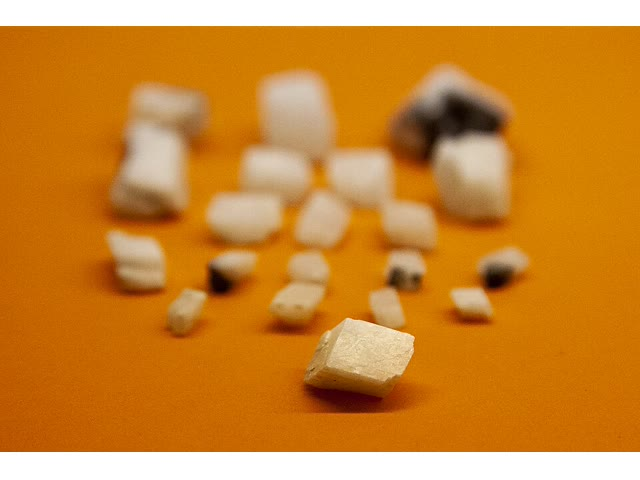
\includegraphics[width=\linewidth]{images/book3/b1-mineral-calcite-rhombs.jpg}

{\scriptsize Calcite cleavage rhombohedra. Photograph Giovanna Canu and Eva
Santini, CC BY 4.0 (Wikimedia Commons).}
\end{minipage}
\end{inthelab}

\begin{omfigure}
\setlength{\tabcolsep}{2pt}
\begin{tabular}{ccc}
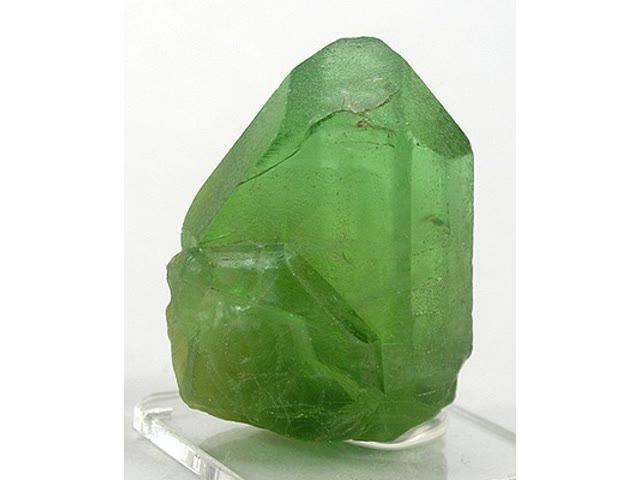
\includegraphics[width=0.31\linewidth]{images/book3/b1-mineral-olivine.jpg} &
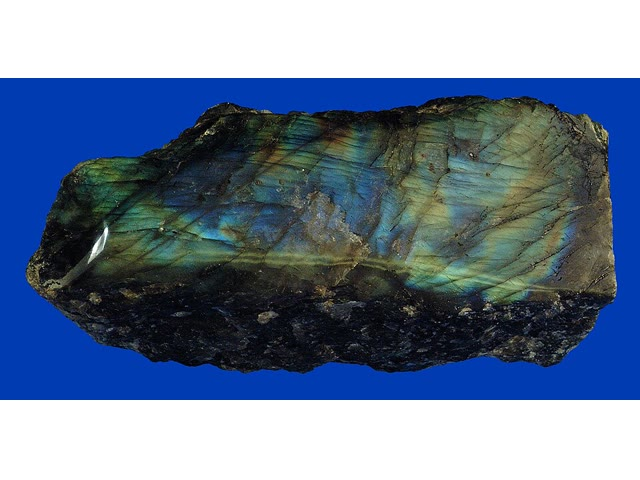
\includegraphics[width=0.31\linewidth]{images/book3/b1-mineral-plagioclase.jpg} &
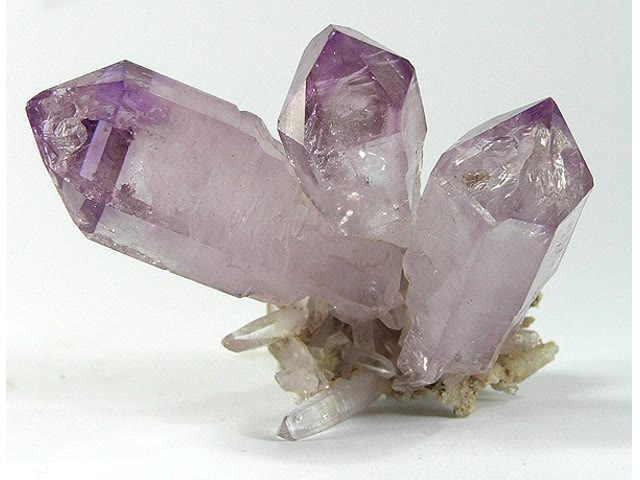
\includegraphics[width=0.31\linewidth]{images/book3/b1-mineral-quartz.jpg} \\
{\small (a) \omterm{def:b1:rock-forming-minerals:groups}{olivine}} & {\small (b) \omterm{def:b1:rock-forming-minerals:groups}{plagioclase} (labradorite)} & {\small (c) quartz (amethyst)} \\[4pt]
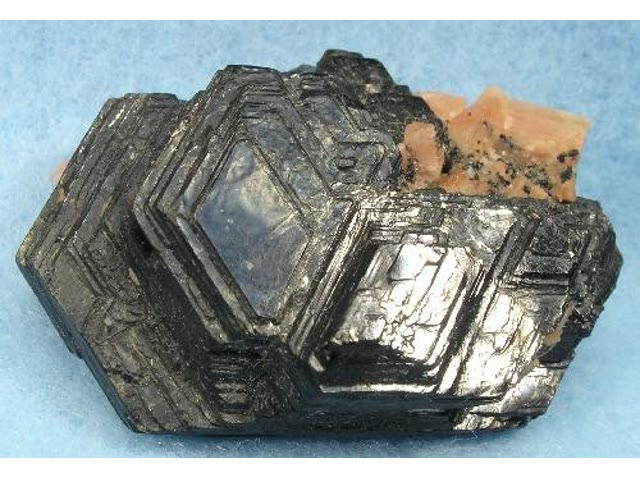
\includegraphics[width=0.31\linewidth]{images/book3/b1-mineral-biotite.jpg} &
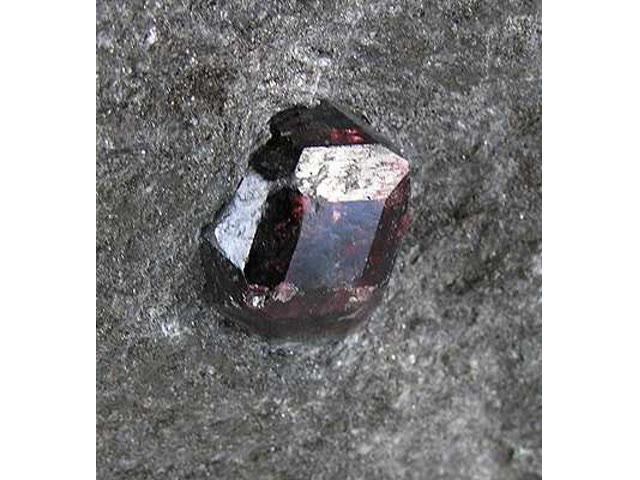
\includegraphics[width=0.31\linewidth]{images/book3/b1-mineral-garnet.jpg} &
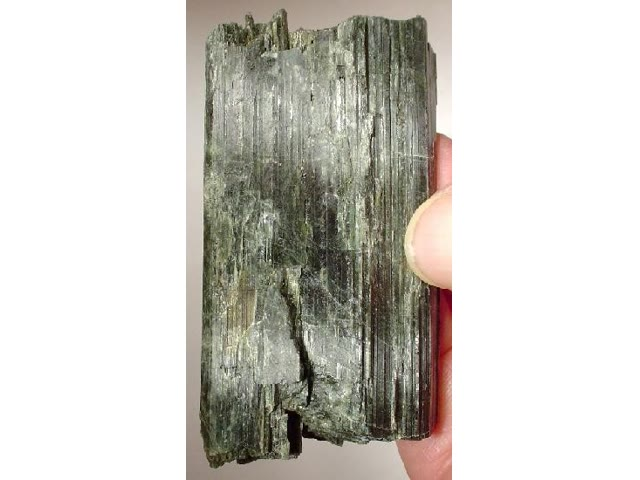
\includegraphics[width=0.31\linewidth]{images/book3/b1-mineral-hornblende.jpg} \\
{\small (d) biotite on orthoclase} & {\small (e) \omterm{def:b1:rock-forming-minerals:groups}{garnet} (almandine)} & {\small (f) hornblende} \\
\end{tabular}
\medskip
% ledger: commons:min-olivine, commons:min-plagioclase, commons:min-quartz, commons:min-biotite, commons:min-garnet, commons:min-hornblende

{\small Six rock-forming \omterm{def:b1:rock-forming-minerals:mineral}{minerals}: (a) a gem \omterm{def:b1:rock-forming-minerals:groups}{olivine} crystal; (b) a polished
slab of \omterm{def:b1:rock-forming-minerals:groups}{plagioclase} showing the play of colours of labradorite; (c) quartz
crystals, six-sided prisms with pyramidal tips; (d) a book of biotite flakes
on a crystal of orthoclase; (e) an almandine \omterm{def:b1:rock-forming-minerals:groups}{garnet} crystal in its
matrix; (f) a prism of hornblende. Photographs (a), (c)--(f) Robert
M.~Lavinsky, CC BY-SA 3.0; (b) Twyla Baker, CC0 (Wikimedia Commons).}
\end{omfigure}

\section{Exercises}

\begin{exercise}[$\star$]\label{exo:b1:rock-forming-minerals:1}
Name the silicate class of each anion, and give the number $s$ of corners
shared by each tetrahedron: \ce{SiO4^{4-}}, \ce{Si2O7^{6-}},
\ce{Si6O18^{12-}}, \ce{Si2O5^{2-}}, \ce{SiO2}. Which class could \ce{SiO3^{2-}}
belong to?
\end{exercise}

\begin{exercise}[$\star$]\label{exo:b1:rock-forming-minerals:2}
With the atomic weights O \num{15.999}, Si \num{28.085}, Mg \num{24.305} and
Fe \qty{55.845}{g.mol^{-1}}, compute the molar masses of forsterite and
fayalite, then their molar volumes from the densities \num{3.275} and
\qty{4.392}{g.cm^{-3}}.
% ledger: ciaaw:O, ciaaw:Si, ciaaw:Mg, ciaaw:Fe, hom:forsterite, hom:fayalite
\end{exercise}

\begin{exercise}[$\star$]\label{exo:b1:rock-forming-minerals:3}
In sixfold coordination the radii are \ce{Mg^{2+}} \qty{0.72}{\angstrom},
\ce{Fe^{2+}} \qty{0.78}{\angstrom}, \ce{Ni^{2+}} \qty{0.69}{\angstrom},
\ce{Mn^{2+}} \qty{0.83}{\angstrom} and \ce{Ca^{2+}} \qty{1.00}{\angstrom}.
Compute the difference of each from the radius of \ce{Mg^{2+}} in per cent,
and say, by Goldschmidt's rules, which can replace magnesium freely in
\omterm{def:b1:rock-forming-minerals:groups}{olivine}.
% ledger: shannon:radii, goldschmidt:size
\end{exercise}

\begin{exercise}[$\star$]\label{exo:b1:rock-forming-minerals:4}
Graphite and diamond have densities \num{2.16} and \qty{3.51}{g.cm^{-3}};
calcite and aragonite \num{2.71} and \qty{2.93}{g.cm^{-3}}. By how many per
cent is the density raised in each change? Which \omterm{def:b1:rock-forming-minerals:polymorph}{polymorph} of each pair forms
at the higher pressure?
% ledger: webmineral:polymorphs, hom:calcite
\end{exercise}

\begin{exercise}[$\star\star$]\label{exo:b1:rock-forming-minerals:5}
Write the \omterm{def:b1:rock-forming-minerals:formula}{structural formula} of the \omterm{def:b1:rock-forming-minerals:groups}{plagioclase} $\text{An}_{30}$ (\qty{30}{\percent}
of the large sites filled by calcium), and check that it is neutral.
\end{exercise}

\begin{exercise}[$\star\star$]\label{exo:b1:rock-forming-minerals:6}
In a double chain, half the tetrahedra share two corners and half share
three. Count the oxygens of a repeating group of four tetrahedra directly on
panel (f) of the linkage figure, and check the formula \ce{Si4O11^{6-}} given by
\cref{prop:b1:rock-forming-minerals:si-o}.
\end{exercise}

\begin{exercise}[$\star\star$]\label{exo:b1:rock-forming-minerals:7}
Recalculate on four oxygens the \omterm{def:b1:rock-forming-minerals:groups}{olivine} analysis \qty{40.20}{\percent}
\ce{SiO2}, \qty{47.10}{\percent} \ce{MgO}, \qty{12.20}{\percent} \ce{FeO},
\qty{0.40}{\percent} \ce{NiO} (molar mass of \ce{NiO}
\qty{74.692}{g.mol^{-1}}).
Give its \omterm{def:b1:rock-forming-minerals:formula}{structural formula}, check it, and give its forsterite content.
Then show that the forsterite content can be found from the \ce{MgO} and
\ce{FeO} percentages alone.
\end{exercise}

\begin{exercise}[$\star\star$]\label{exo:b1:rock-forming-minerals:8}
Check that muscovite \ce{KAl2(Si3Al)O10(OH)2} is neutral. Its sheets of
tetrahedra have one aluminium for three silicons: what charge does this give
the sheet per formula unit, and which ion balances it?
\end{exercise}

\begin{exercise}[$\star\star$]\label{exo:b1:rock-forming-minerals:9}
Using the molar volumes \num{42.96} and \qty{46.40}{cm^3.mol^{-1}} and the
molar masses \num{140.691} and \qty{203.771}{g.mol^{-1}}: (a) compute the
density of $\text{Fo}_{50}$ by ideal mixing, and compare it with the mean of the
\omterm{def:b1:rock-forming-minerals:solid-solution}{end-member} densities; (b) find the forsterite content of an \omterm{def:b1:rock-forming-minerals:groups}{olivine} of
density \qty{3.600}{g.cm^{-3}}.
\end{exercise}

\begin{exercise}[$\star\star\star$]\label{exo:b1:rock-forming-minerals:10}
With the notation of \cref{prop:b1:rock-forming-minerals:ideal-mixing}, show
that
\[
  \rho(x) - \bigl(x\rho_1 + (1 - x)\rho_2\bigr) =
  \frac{x(1 - x)(\rho_1 - \rho_2)(V_1 - V_2)}{V(x)} .
\]
Deduce that the density of \omterm{def:b1:rock-forming-minerals:groups}{olivine} lies above the straight line between the
\omterm{def:b1:rock-forming-minerals:solid-solution}{end-members}, and compute the gap at $\text{Fo}_{50}$.
\end{exercise}

\begin{exercise}[$\star\star\star$]\label{exo:b1:rock-forming-minerals:11}
A \omterm{def:b1:rock-forming-minerals:groups}{plagioclase} from a gabbro gives \qty{54.10}{\percent} \ce{SiO2},
\qty{28.90}{\percent} \ce{Al2O3}, \qty{11.20}{\percent} \ce{CaO},
\qty{5.10}{\percent} \ce{Na2O} and \qty{0.30}{\percent} \ce{K2O} (molar
masses \num{60.083}, \num{101.961}, \num{56.077}, \num{61.979},
\qty{94.195}{g.mol^{-1}}). Recalculate it on eight oxygens; check that the
tetrahedral sites (Si + Al) hold 4 atoms and the large site
(Ca + Na + K) 1; check the \omterm{def:b1:rock-forming-minerals:substitution}{coupled substitution} by comparing $\mathrm{Al} - 1$
with Ca; give the anorthite content $100\,\mathrm{Ca}/(\mathrm{Ca} +
\mathrm{Na} + \mathrm{K})$.
\end{exercise}

\begin{exercise}[$\star\star\star$]\label{exo:b1:rock-forming-minerals:12}
A microprobe cannot tell \ce{Fe^{2+}} from \ce{Fe^{3+}} and reports all iron
as \ce{FeO}. (a) Show that pure magnetite \ce{Fe3O4}, analysed this way,
totals \qty{93.09}{\percent}. (b) Recalculate this analysis on four oxygens,
and say why the result is impossible for a \omterm{def:b1:rock-forming-minerals:mineral}{mineral} with three cations per four
oxygens. (c) Recalculate on three cations instead, and find the numbers of
\ce{Fe^{2+}} and \ce{Fe^{3+}} by requiring the formula to be neutral.
(d) Re-express the analysis as \ce{FeO} and \ce{Fe2O3}, and give the new
total.
\end{exercise}

\section{Problem: An olivine from a basalt}

\begin{problem}[{Weekend problem --- recalculating a microprobe analysis of an
olivine, writing and checking its formula, and finding its composition, its
density and its mass in a cubic metre of basalt}]
\label{pb:b1:rock-forming-minerals:1}
% invented analysis: figdata/bachelor-1/solid_solution.py (OLIVINE_WT); values: calc/ch07.py
% ledger: ciaaw:O, ciaaw:Si, ciaaw:Mg, ciaaw:Fe, ciaaw:Mn, ciaaw:Ni, ciaaw:Ca, hom:forsterite, hom:fayalite, shannon:radii
The green crystals of a basalt are \omterm{def:b1:rock-forming-minerals:groups}{olivine}. A microprobe analysis of one of
them gives, in weight per cent of oxides:
\begin{center}
\small
\begin{tabular}{lcccccc}
\hline
oxide & \ce{SiO2} & \ce{FeO} & \ce{MnO} & \ce{MgO} & \ce{NiO} & \ce{CaO} \\
weight \% & 39.50 & 16.53 & 0.23 & 43.32 & 0.20 & 0.22 \\
\hline
\end{tabular}
\end{center}
The atomic weights are O \num{15.999}, Si \num{28.085}, Fe \num{55.845}, Mn
\num{54.938}, Mg \num{24.305}, Ni \num{58.693}, Ca \qty{40.078}{g.mol^{-1}}.
Forsterite has density \qty{3.275}{g.cm^{-3}} and fayalite
\qty{4.392}{g.cm^{-3}}.

\medskip
\noindent\textbf{Part I --- From oxides to cations.}
\begin{enumerate}
  \item Compute the molar masses of the six oxides.
  \item Compute the total of the analysis. What would a total of
        \qty{97}{\percent} have suggested?
  \item Compute the number of moles of each oxide in \qty{100}{g} of
        \omterm{def:b1:rock-forming-minerals:groups}{olivine}.
  \item Compute the moles of oxygen they contain, and their sum.
  \item Compute the moles of each cation.
  \item Compute the factor that brings the oxygens to four.
  \item Give the number of atoms of each element per four oxygens, to three
        decimals.
\end{enumerate}

\medskip
\noindent\textbf{Part II --- The structural formula.}
\begin{enumerate}[resume]
  \item \omterm{def:b1:rock-forming-minerals:groups}{Olivine} has one tetrahedral site and two octahedral sites per four
        oxygens. Compute the sum of the cations other than silicon, and
        compare both site totals with the ideal formula.
  \item Write the \omterm{def:b1:rock-forming-minerals:formula}{structural formula} of the \omterm{def:b1:rock-forming-minerals:groups}{olivine}.
  \item Check that the formula is neutral, and explain why this check,
        unlike that of question 8, could not have failed.
  \item Using the ionic radii (\ce{Mg^{2+}} \qty{0.72}{\angstrom},
        \ce{Fe^{2+}} \qty{0.78}{\angstrom}, \ce{Ni^{2+}}
        \qty{0.69}{\angstrom}, \ce{Mn^{2+}} \qty{0.83}{\angstrom},
        \ce{Ca^{2+}} \qty{1.00}{\angstrom}, all sixfold), explain why nickel
        is common in \omterm{def:b1:rock-forming-minerals:groups}{olivine} and calcium rare.
  \item The probe reports all iron as \ce{FeO}. Explain why the total number
        of cations found in question 7 shows that the \omterm{def:b1:rock-forming-minerals:groups}{olivine} contains no
        significant \ce{Fe^{3+}}.
\end{enumerate}

\medskip
\noindent\textbf{Part III --- The composition.}
\begin{enumerate}[resume]
  \item Compute the forsterite content $\mathrm{Fo} = 100\,\mathrm{Mg}/(\mathrm{Mg} +
        \mathrm{Fe})$, to one decimal.
  \item What is the \omterm{def:b1:rock-forming-minerals:formula}{Mg number} of the \omterm{def:b1:rock-forming-minerals:groups}{olivine}? Why is it equal to the
        forsterite content here?
  \item Write the \omterm{def:b1:rock-forming-minerals:groups}{olivine} as a binary \omterm{def:b1:rock-forming-minerals:solid-solution}{solid solution}
        $\mathrm{Fo}_x\mathrm{Fa}_{1-x}$, ignoring Mn, Ni and Ca, and give the
        proportion of its octahedral sites holding iron.
  \item Show that the forsterite content can be computed from the
        \ce{MgO} and \ce{FeO} percentages alone, without the factor of
        question 6, and do it.
  \item An \omterm{def:b1:rock-forming-minerals:groups}{olivine} that grew later in the same lava has \qty{40.5}{\percent}
        \ce{MgO} and \qty{20.0}{\percent} \ce{FeO}. Compute its forsterite
        content. Which \omterm{def:b1:rock-forming-minerals:groups}{olivine} is richer in iron?
\end{enumerate}

\medskip
\noindent\textbf{Part IV --- Density and mass.}
\begin{enumerate}[resume]
  \item Compute the molar masses and the molar volumes of forsterite and
        fayalite (molar volumes to two decimals).
  \item Taking the \omterm{def:b1:rock-forming-minerals:groups}{olivine} as the binary $\mathrm{Fo}_x\mathrm{Fa}_{1-x}$ of
        question 15, with $x$ rounded to three decimals, compute its molar
        mass and its molar volume by ideal mixing.
  \item Deduce its density, to three decimals.
  \item Compare it with the straight-line interpolation between the
        \omterm{def:b1:rock-forming-minerals:solid-solution}{end-member} densities.
  \item The basalt contains \qty{12}{\percent} \omterm{def:b1:rock-forming-minerals:groups}{olivine} by volume. What mass
        of \omterm{def:b1:rock-forming-minerals:groups}{olivine} does a cubic metre of the basalt contain?
  \item The basalt has a density of \qty{2.95}{g.cm^{-3}}. What is the
        proportion of \omterm{def:b1:rock-forming-minerals:groups}{olivine} by mass?
  \item What is the forsterite content of the \omterm{def:b1:rock-forming-minerals:groups}{olivine}, rounded to the whole
        per cent?
\end{enumerate}
\end{problem}
